\chapter{Validation et évaluation}
\label{chap:validation}

\section{Stratégie de test}

La validation combine quatre niveaux complémentaires :

\begin{description}[style=nextline,leftmargin=1em]
  \item[Tests fonctionnels.] Exécution des programmes de démonstration et
        comparaison des sorties avec les résultats attendus.
  \item[Tests de gestion d'erreurs.] Soumission de programmes fautifs pour
        vérifier que chaque catégorie d'erreur est détectée, localisée et
        signalée.
  \item[Tests de non-régression.] Après chaque évolution (optimisations,
        extensions, corrections), re-vérification que les sorties de référence
        restent identiques.
  \item[Tests de robustesse mémoire et cas limites.] Analyse Valgrind et
        campagne de cas extrêmes (fichier vide, EOF, grands nombres, récursion
        profonde, ruptures de flot mal placées).
\end{description}

\section{Protocole expérimental}

\subsection{Conditions et métriques}

Les mesures de performance ont été réalisées sur une machine équipée d'un
processeur AMD Ryzen~5 5500 (12 fils d'exécution), sous Ubuntu (WSL). Chaque temps
rapporté est le \emph{meilleur} de trois exécutions (pour limiter le bruit lié à
l'ordonnancement), mesuré par \code{/usr/bin/time}. Les métriques retenues sont :
le temps d'exécution (secondes), le résultat calculé (pour la correction), et le
verdict Valgrind (octets perdus, erreurs).

\subsection{Jeux d'essai}

Les programmes de démonstration servent de jeu d'essai fonctionnel : Fibonacci
récursif, PGCD d'Euclide, programme interactif, plus les deux programmes
illustrant les extensions (flottants, boucles avec \code{arrêter}/\code{continuer}).
Les benchmarks utilisent des programmes paramétrés (Fibonacci à différentes
tailles, boucle de 30~millions d'itérations, récursion profonde).

\subsection{Reproductibilité}

Les tests sont automatisés et rejouables. La cible \code{make test} compile puis
exécute l'ensemble des programmes de démonstration ; un script dédié soumet les
programmes fautifs et affiche, pour chacun, le message d'erreur et le code de
sortie. Ce script tient en quelques lignes et illustre bien la simplicité du
dispositif :

\begin{lstlisting}[style=gram,caption={C\oe ur du script de test des erreurs.}]
for f in variable divzero fonction arguments lexical syntaxe; do
    echo "===== $f ====="
    ./ilang "tests/err_$f.ilang"   # le programme fautif
    echo "(code de sortie : $?)"   # 1 si erreur fatale, 0 si poursuite
done
\end{lstlisting}

Cette automatisation a servi de filet de sécurité tout au long du développement.
Après chaque modification, une simple commande permettait de vérifier qu'aucune
sortie de référence n'avait changé. C'est précisément ce dispositif qui m'a permis
de garantir la non-régression lors de l'ajout des flottants, puis des deux autres
extensions, puis du back-end assembleur, sans craindre de casser silencieusement
ce qui fonctionnait déjà.

\section{Résultats fonctionnels}

\subsection{Programmes de démonstration}

Les trois programmes du cahier des charges produisent les sorties attendues.

\begin{lstlisting}[style=ilang,caption={Sortie de \code{fibonacci.ilang} (15 premiers termes).}]
0 1 1 2 3 5 8 13 21 34 55 89 144 233 377
\end{lstlisting}

\begin{lstlisting}[style=ilang,caption={Sortie de \code{pgcd.ilang} : pgcd(48, 18).}]
6
\end{lstlisting}

\begin{lstlisting}[style=ilang,caption={Sortie de \code{interactif.ilang} pour les entrées 7 puis $-5$.}]
999      999
49       5
\end{lstlisting}

Les programmes d'extension confirment le bon fonctionnement des flottants et des
ruptures de boucle :

\begin{lstlisting}[style=ilang,caption={Sortie de \code{flottants.ilang}.}]
6.28      (3.14 * 2)
3.5       (2.5 + 1)
2         (10 / 4   : division entiere preservee)
2.5       (10.0 / 4 : division reelle)
19.6349   (aire d'un disque de rayon 2.5)
1         (3.5 > 3)
\end{lstlisting}

\begin{lstlisting}[style=ilang,caption={Sortie de \code{boucles.ilang} (arrêter puis continuer puis arrêter dans un tant que).}]
0 1 2 3 4        (arret a 5)
1 3 5 7 9        (saut des pairs)
10 9 8           (arret a 7)
\end{lstlisting}

\subsection{Gestion des erreurs}

Chaque catégorie d'erreur du cahier des charges est traitée et localisée à la
ligne (tableau~\ref{tab:erreurs}). Cas notable, la division par zéro émet un
message \emph{et laisse le programme continuer}, conformément à la spécification.

\begin{table}[ht]
\centering
\caption{Gestion des erreurs : message émis et code de sortie.}
\label{tab:erreurs}
\small
\begin{tabular}{@{}lll@{}}
\toprule
\textbf{Erreur} & \textbf{Message} & \textbf{Sortie} \\
\midrule
Variable non définie & \code{Erreur ligne 1 : variable 'z' non definie} & 1 \\
Division par zéro & \code{Erreur ligne 1 : division par zero} & 0 (continue) \\
Fonction non définie & \code{Erreur ligne 1 : fonction 'inconnue' non definie} & 1 \\
Mauvais nb d'arguments & \code{... attend 2 argument(s), 1 fourni(s)} & 1 \\
Caractère invalide & \code{Erreur lexicale ligne 1 : caractere invalide '@'} & 1 \\
Erreur de syntaxe & \code{Erreur de syntaxe ligne 1 : syntax error...} & 1 \\
Rupture hors boucle & \code{Erreur ligne 2 : 'arreter' utilise hors d'une boucle} & 1 \\
\bottomrule
\end{tabular}
\end{table}

Pour illustrer concrètement le traitement des erreurs, voici les sorties réelles
produites par l'interpréteur sur une série de programmes fautifs. On notera la
localisation systématique à la ligne et, pour la division par zéro, la poursuite
de l'exécution.

\begin{lstlisting}[style=gram,caption={Sorties réelles sur des programmes fautifs.}]
$ ./ilang tests/err_variable.ilang
Erreur ligne 1 : variable 'z' non definie

$ ./ilang tests/err_divzero.ilang
Erreur ligne 1 : division par zero
0
123                  <- le programme continue apres l'erreur

$ ./ilang tests/err_fonction.ilang
Erreur ligne 1 : fonction 'inconnue' non definie

$ ./ilang tests/err_arguments.ilang
Erreur ligne 5 : fonction 'pgcd' attend 2 argument(s), 1 fourni(s)

$ ./ilang tests/err_lexical.ilang
Erreur lexicale ligne 1 : caractere invalide '@'

$ ./ilang tests/err_syntaxe.ilang
Erreur de syntaxe ligne 1 : syntax error, unexpected IDENTIFIANT, expecting '('
\end{lstlisting}

\section{Résultats de performance}

\subsection{Interprétation contre code natif}

Le tableau~\ref{tab:bench-fib} et la figure~\ref{fig:bench-fib} comparent le temps
de calcul de Fibonacci par l'interpréteur et par le binaire issu du back-end
assembleur. L'écart est spectaculaire : sur \code{fib(32)}, le code natif est de
l'ordre de \emph{plusieurs centaines de fois} plus rapide. Cela illustre
concrètement le coût du parcours d'arbre (distribution sur le type de n\oe ud,
appels de fonction C en cascade) face à du code machine compilé.

\begin{table}[ht]
\centering
\caption{Temps d'exécution de Fibonacci : interpréteur vs assembleur i386.}
\label{tab:bench-fib}
\begin{tabular}{@{}rrrr@{}}
\toprule
$n$ & résultat & interpréteur (s) & asm i386 (s) \\
\midrule
28 & 317\,811   & 0,43 & $\approx$ 0,00 \\
30 & 832\,040   & 1,13 & $\approx$ 0,00 \\
32 & 2\,178\,309 & 2,97 & 0,01 \\
\bottomrule
\end{tabular}
\end{table}

\begin{figure}[ht]
\centering
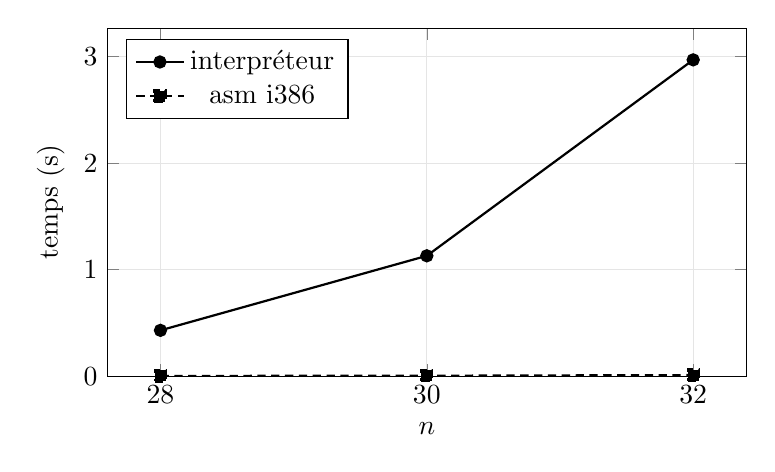
\begin{tikzpicture}
\begin{axis}[
  width=0.8\textwidth, height=6cm,
  xlabel={$n$}, ylabel={temps (s)},
  legend pos=north west,
  xtick={28,30,32},
  ymin=0, grid=both, grid style={black!10},
]
\addplot[mark=*,thick] coordinates {(28,0.43) (30,1.13) (32,2.97)};
\addplot[mark=square*,thick,densely dashed] coordinates {(28,0.002) (30,0.004) (32,0.01)};
\legend{interpréteur, asm i386}
\end{axis}
\end{tikzpicture}
\caption{Croissance du temps d'exécution de Fibonacci. La courbe de
l'interpréteur révèle bien la complexité exponentielle de l'algorithme ; le code
natif, sur la même échelle, reste collé à l'axe.}
\label{fig:bench-fib}
\end{figure}

\subsection{Effet des optimisations}

Pour isoler l'effet du pliage de constantes, un programme effectue 30~millions
d'itérations d'un corps de boucle contenant une expression constante
(\code{s = s + (2*3 + 4*5 - 6)}, qui se replie en \code{s + 20}). Le drapeau
\code{--no-opt} permet de désactiver l'optimiseur. Le pliage fait gagner environ
un tiers du temps (figure~\ref{fig:bench-opt}).

\begin{figure}[ht]
\centering
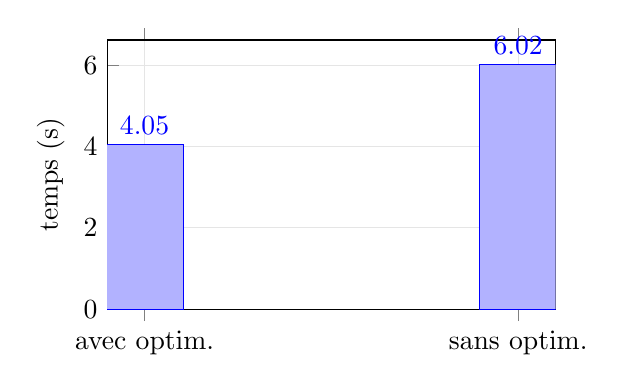
\begin{tikzpicture}
\begin{axis}[
  width=0.6\textwidth, height=5cm,
  ybar, bar width=28pt,
  symbolic x coords={avec optim., sans optim.},
  xtick=data, ymin=0,
  ylabel={temps (s)}, nodes near coords,
  grid=both, grid style={black!10},
]
\addplot coordinates {(avec optim.,4.05) (sans optim.,6.02)};
\end{axis}
\end{tikzpicture}
\caption{Temps de la boucle de 30~M d'itérations, avec et sans pliage de
constantes. Le gain ($\approx$ 33~\%) provient de la suppression du calcul
arithmétique répété à chaque tour.}
\label{fig:bench-opt}
\end{figure}

\subsection{Limite de profondeur de récursion}

Comme l'évaluateur récurse en C (un appel \ilang{} se traduit par une cascade
d'appels de \code{eval}), la profondeur de récursion est bornée par la pile de
l'hôte. La sonde du tableau~\ref{tab:rec} montre que \code{somme(5000)} aboutit,
mais que \code{somme(10000)} provoque un débordement de pile (signal SIGSEGV,
code de sortie 139). C'est une limite de fond de l'approche par parcours d'arbre,
discutée au chapitre~\ref{chap:discussion}.

\begin{table}[ht]
\centering
\caption{Profondeur de récursion : \code{somme(n)} récursive.}
\label{tab:rec}
\begin{tabular}{@{}rl@{}}
\toprule
$n$ & résultat \\
\midrule
1\,000  & 500\,500 (ok) \\
5\,000  & 12\,502\,500 (ok) \\
10\,000 & débordement de pile (SIGSEGV) \\
\bottomrule
\end{tabular}
\end{table}

\subsection{Vérification mémoire}

L'exécution sous Valgrind, après ajout de \code{yylex\_destroy()}, ne signale
\textbf{aucune fuite ni erreur} sur l'ensemble des programmes :

\begin{lstlisting}[style=gram,caption={Verdict Valgrind (programme \code{pgcd.ilang}).}]
in use at exit: 0 bytes in 0 blocks
ERROR SUMMARY: 0 errors from 0 contexts (suppressed: 0 from 0)
\end{lstlisting}

\subsection{Équivalence interpréteur / code généré}

Enfin, pour chaque programme entier, la sortie du binaire assemblé a été comparée
à celle de l'interpréteur : elles sont \textbf{identiques} (Fibonacci, PGCD,
boucles avec \code{arrêter}/\code{continuer}, et même le programme interactif qui
passe par \code{scanf}/\code{printf}). Le back-end refuse proprement les
programmes utilisant des flottants. Cette équivalence constitue une validation
croisée précieuse : deux back-ends indépendants, partant du même AST, calculent
les mêmes résultats.

\section{Étude de cas de bout en bout}

Pour conclure ce chapitre, suivons le programme \code{factorielle} (présenté au
chapitre~\ref{chap:conception}) tout au long de la chaîne, afin de relier les
résultats aux étapes décrites.

\begin{enumerate}
  \item \textbf{Analyse lexicale.} Le source est découpé en tokens :
        \code{FONCTION}, \code{IDENTIFIANT(factorielle)}, \code{'('},
        \code{IDENTIFIANT(n)}, \code{')'}, \code{'\{'}, \code{SI}, \dots{} Les
        commentaires et espaces sont éliminés.
  \item \textbf{Analyse syntaxique.} Bison réduit ces tokens selon la grammaire et
        bâtit l'AST : une \code{NODE\_FUNC\_DECL} (paramètre \code{n}, corps
        contenant un \code{NODE\_IF} et un \code{NODE\_RETURN} avec un
        \code{NODE\_BINOP} \code{*} dont le fils droit est un
        \code{NODE\_FUNC\_CALL} récursif).
  \item \textbf{Optimisation.} Le sous-arbre \code{n - 1} n'est pas constant (il
        dépend de \code{n}) : rien n'est plié ici, la passe laisse l'arbre
        inchangé, ce qui est correct.
  \item \textbf{Évaluation.} La fonction est d'abord enregistrée (pré-passe), puis
        la boucle \code{pour} appelle \code{factorielle(1)} à
        \code{factorielle(5)}. Chaque appel empile un frame, lie \code{n}, évalue
        le corps, et dépile. Les valeurs retournées sont 1, 2, 6, 24, 120.
  \item \textbf{Sortie.} \code{afficher} imprime chaque résultat :
\end{enumerate}

\begin{lstlisting}[style=gram]
$ ./ilang factorielle.ilang
1
2
6
24
120
\end{lstlisting}

\noindent Le même programme passé à \code{./ilang -s} produit l'assembleur de
l'annexe~\ref{annexe:asm} qui, compilé et exécuté, affiche exactement la même
chose. La boucle complète, depuis le texte source jusqu'au résultat et par deux
back-ends indépendants, est ainsi vérifiée de bout en bout.
